\documentclass[UTF8]{ctexart}
\usepackage{geometry}
\usepackage{graphicx}
\usepackage[namelimits]{amsmath} %数学公式
\usepackage{amssymb}             %数学公式             %数学字体
\usepackage{mathrsfs} 
\usepackage{txfonts}
\usepackage{float}  %设置图片浮动位置的宏包
\usepackage{subfigure}%插入多图时用子图显示的宏包
\geometry{a4paper,scale=0.80}
\author{左熙辰-2000012103}
\date{}
\title{植物学实验1}
\ctexset{
    section/name= {实验操作}
}
\begin{document}
\section{被子植物生殖结构的形态结构与发育}
\begin{figure}[h]
    \centering
    \subfigure[雌性生殖系统]{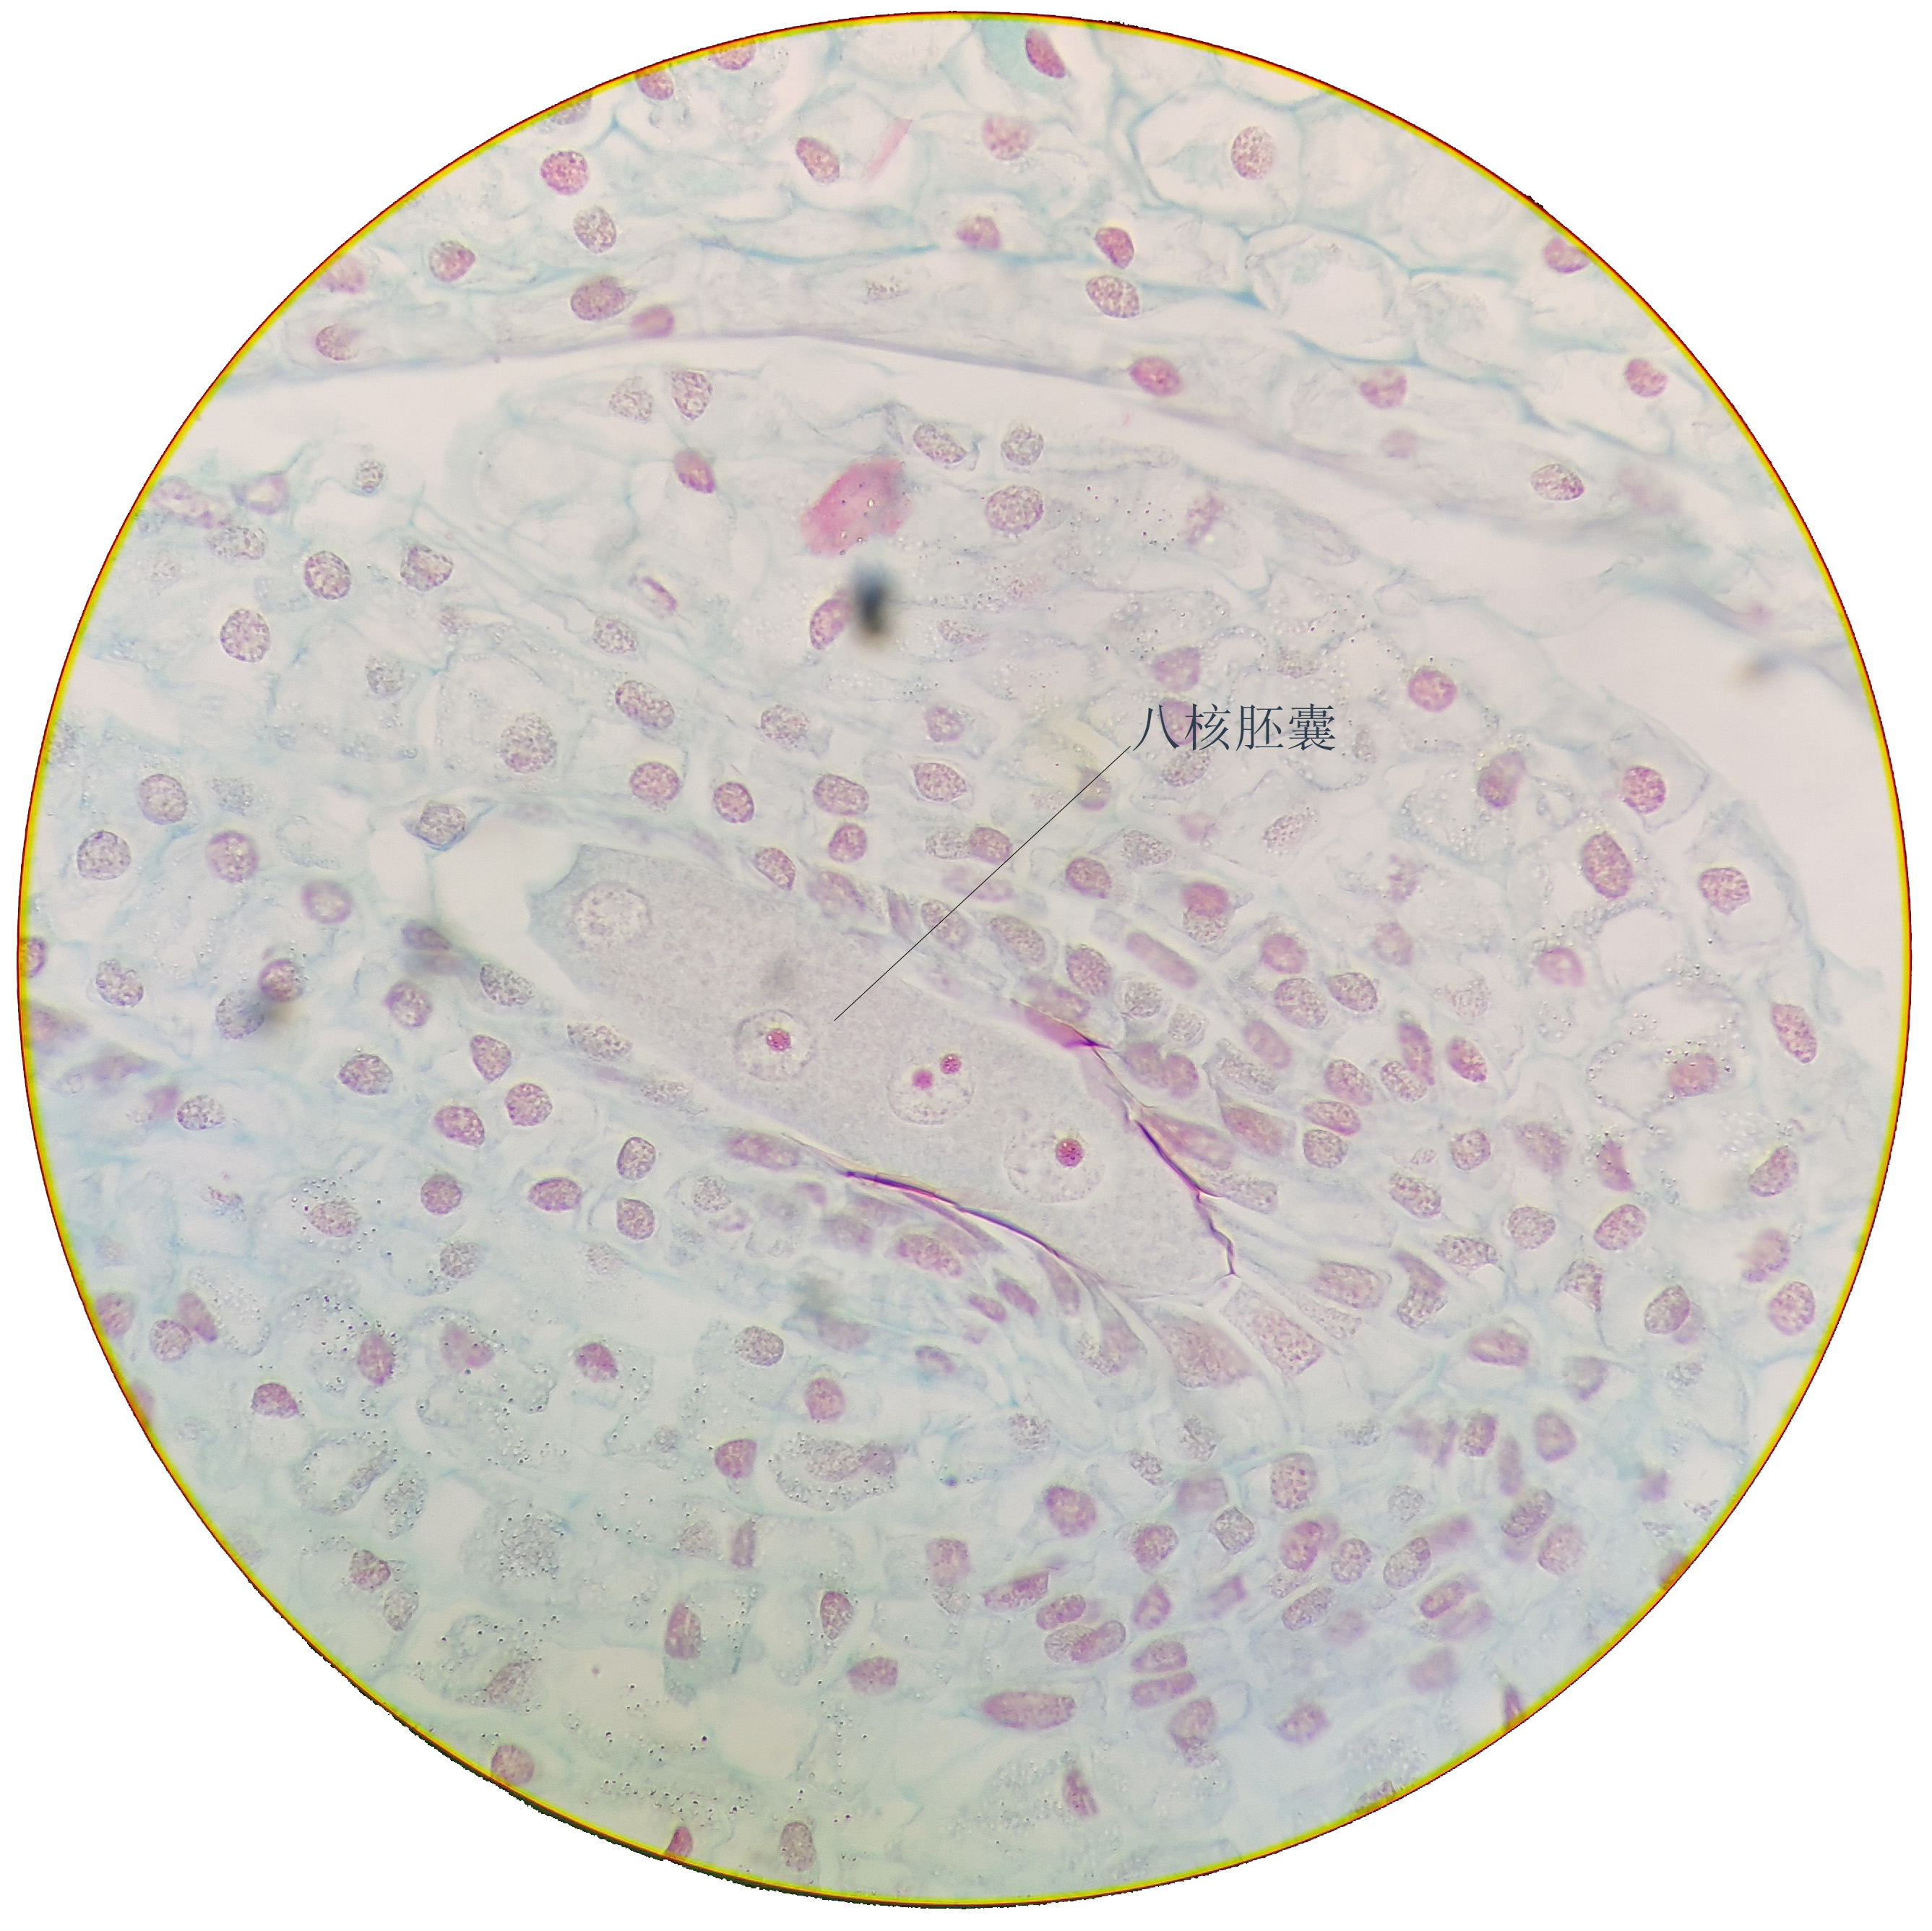
\includegraphics[scale=0.08]{src/botany/微信图片_20201218171753.jpg}\ref{ci}}
    \subfigure[雄性生殖系统]{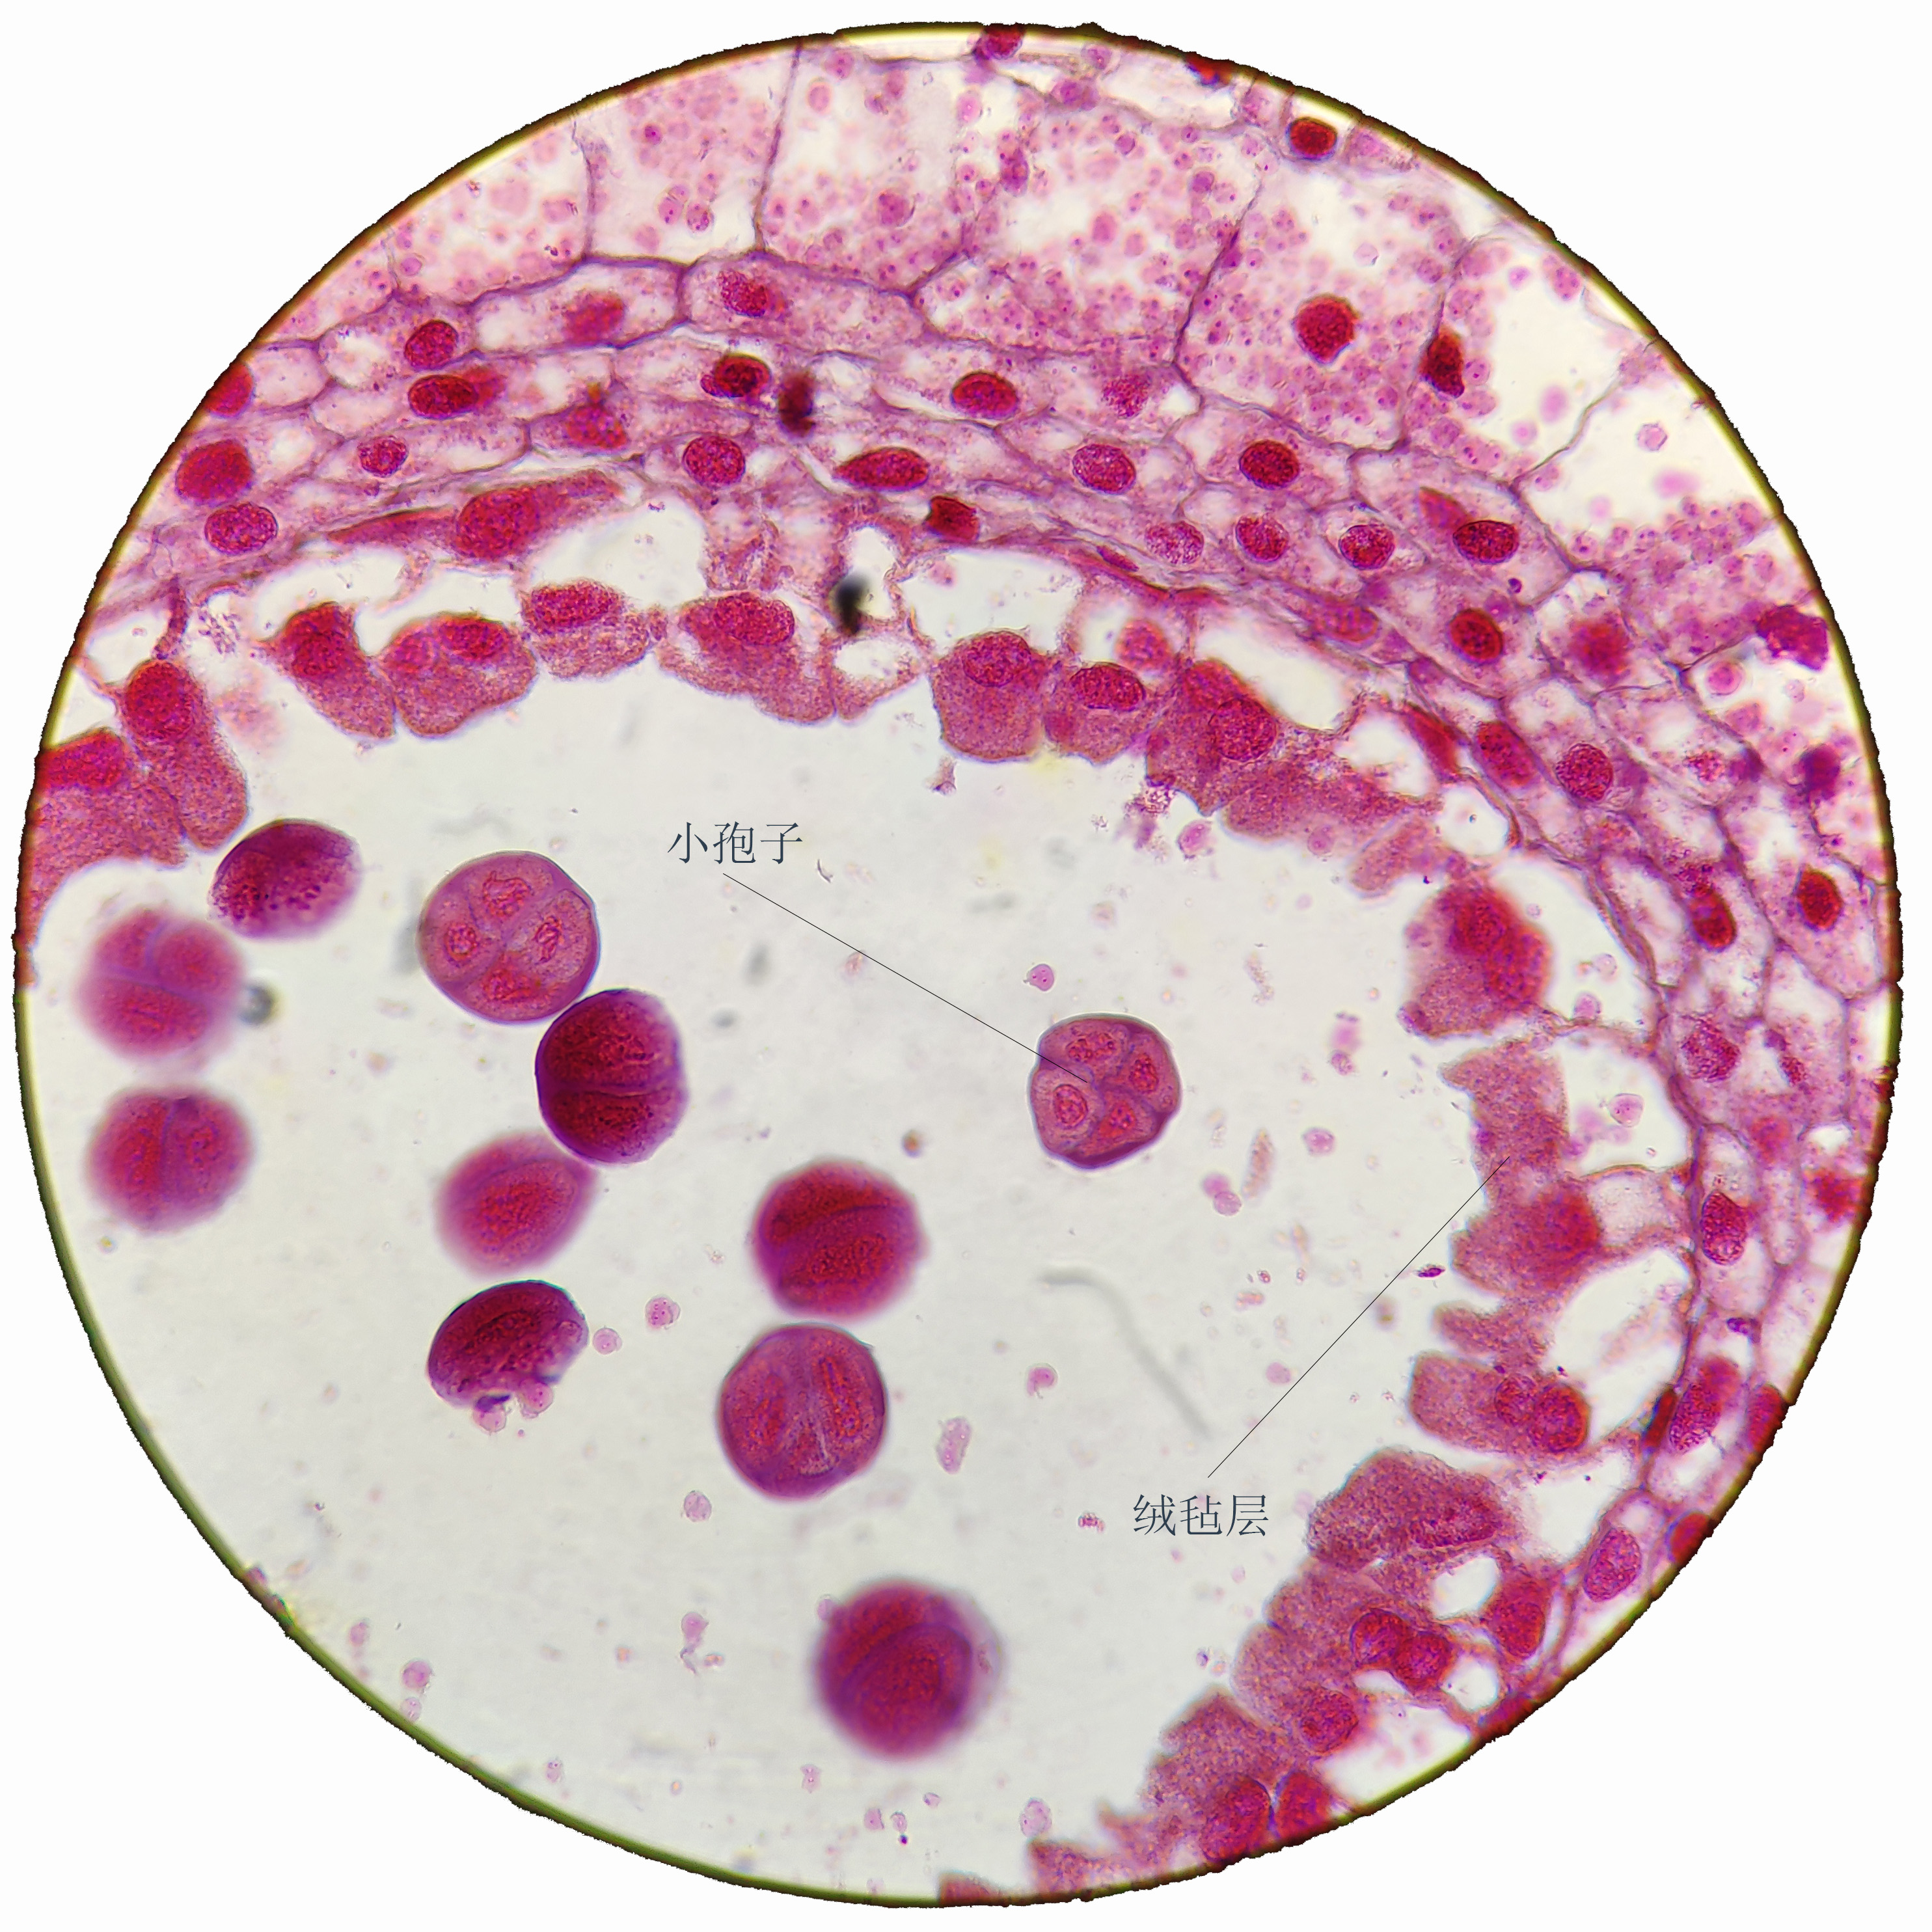
\includegraphics[scale=0.08]{src/botany/微信图片_20201218171731.jpg}\ref{xiong}}
    \caption{被子植物生殖结构的形态结构}
\end{figure}
\begin{figure}[h]
    \centering
    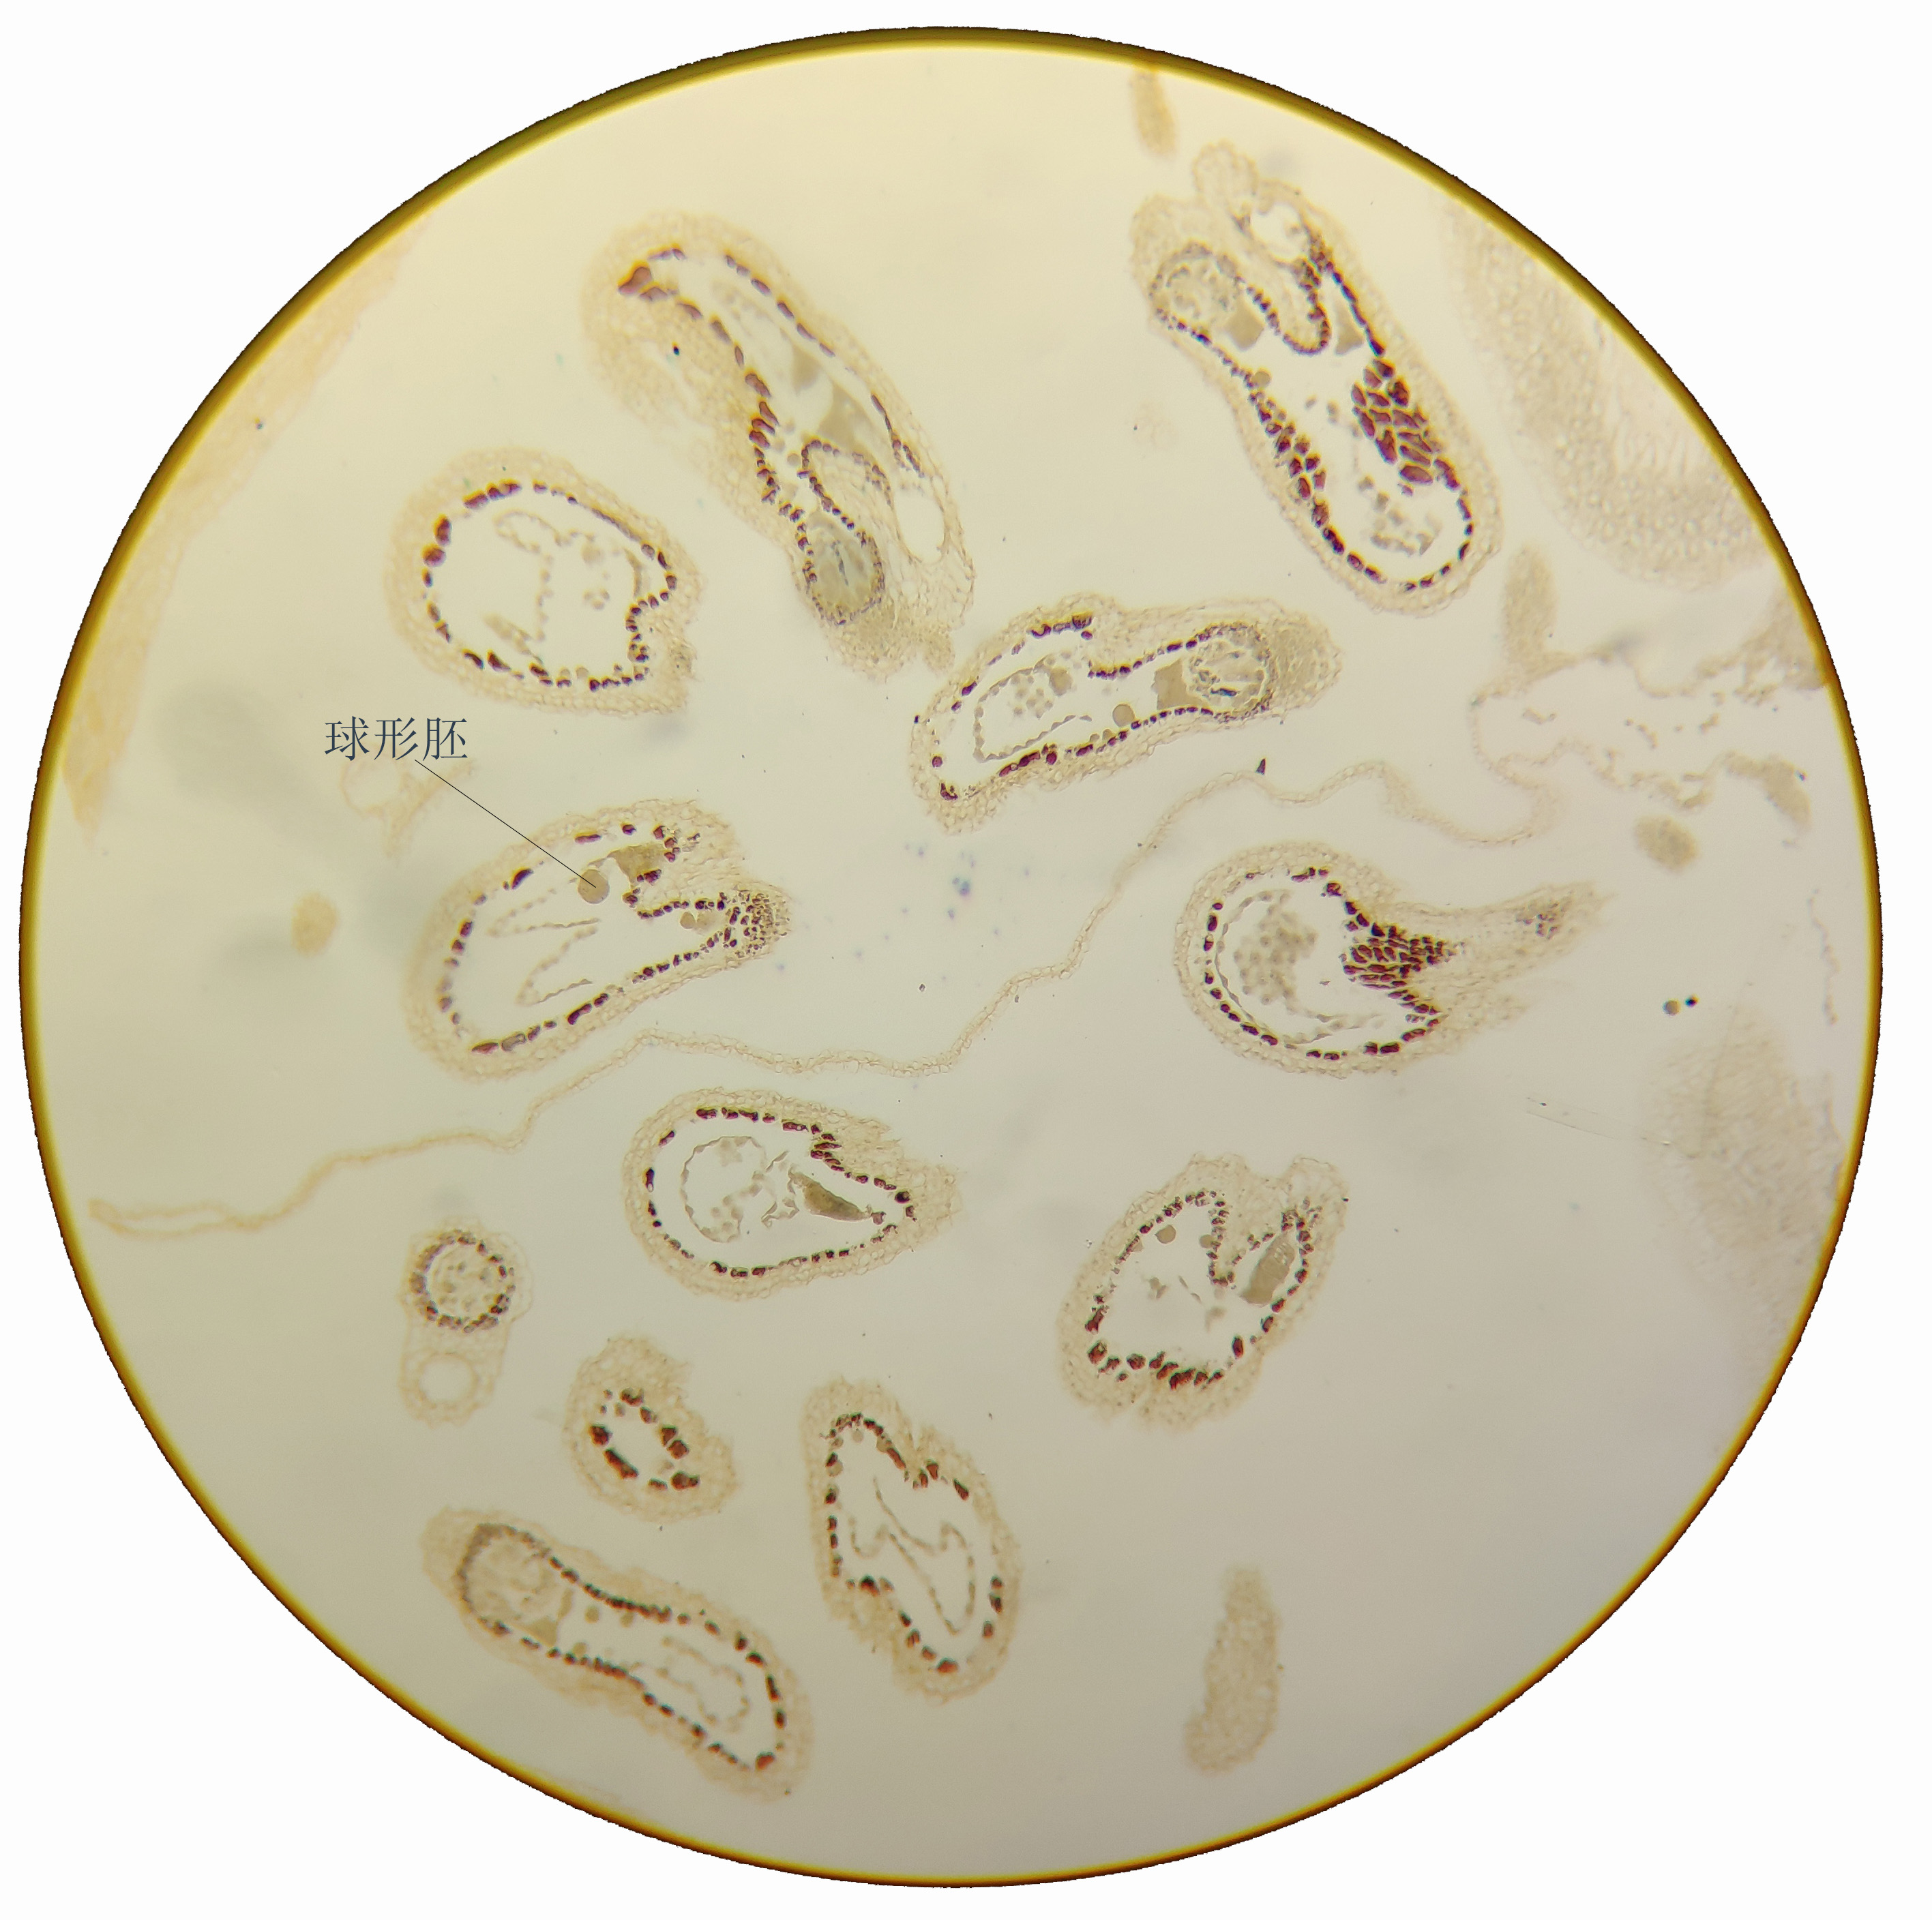
\includegraphics[scale=0.08]{src/botany/微信图片_20201218171809.jpg}
    \label{jicai}
    \caption{荠菜球形胚}
\end{figure}
\paragraph*{写出集中观察的花的花程式}
\paragraph*{答:}长寿花:⚥$\text{⚥}\text{ }\text{*}\text{K}_{(4)}\text{C}_{(4)}\text{A}_{4+4}\underline{\text{G}}_{(4:1:\infty)}$
丝兰:$\text{*}\text{ P}_{3+3}A_{3+3}\underline{\text{G}}_{(3:3:\infty)}$
\paragraph*{2.用简图或照片显示百合雌、雄配子体的结构,并标注出相应的结构名称.}
\paragraph*{答:}见\ref{ci}和\ref{xiong}
\paragraph*{3.用简图或照片显示荠菜球形胚或心形胚时期配囊的结构,并标注出相应的结构名称。}
\paragraph*{答:}见\ref{jicai}
\subsection*{讨论}
\paragraph*{1.根中的凯氏带在什么位置?有什么特点?它的功能是什么?}
\paragraph*{答:}在内皮层外部。四面(或五面)木质化加厚;起控制物质进出的作用
\paragraph*{2. C3植物与C4植物时片结构有什么不同?哪种具有更强的光合作用效率?为什么?}
\paragraph*{答:}C3植物无花环状结构,而C4植物存在。C4。PEP羧化酶$K_{sp}$更低,可以利用更低浓度的CO$_2$
\paragraph*{3.百合的胚乳是几倍体?为什么?}
\paragraph*{答:}五倍体。因为其极核是三倍体
\end{document}